In this section we introduce a family of simplicial complexes that we call \emph{doubly pruned}\footnote{We call these complexes doubly pruned because each complex is a simplex on $[i, j]$ with two pieces cut away: the faces containing an initial interval $[i, p],$ and the faces containing a final interval $[q, j].$}. These are simplicial complexes $\Delta_w$ that are determined by two interval nonfaces and singletons outside of it (\Cref{def: doubly pruned simplicial complexes}). For now, this section will focus on the properties of these complexes that are required in the proofs of the main theorem. In particular, we establish a dictionary between $\sn(\calP)$ and these complexes that match Bruhat order with containment and the closure properties needed to pass from a single permutation to an antichain. 
The combinatorial and homological consequences of these complexes are deferred to \Cref{sec: the combinatorics of doubly pruned simplicial complexes}.

\begin{definition}
\label{def: doubly pruned simplicial complexes}
A simplicial complex $\Delta$ on vertex set $[n]$ is \emph{doubly pruned} if $\Delta = \emptyset$ or for some $1\leq i\leq j\leq n$ its nonfaces are generated by the singletons $\{k\}$ for $k\in[n]\setminus[i,j]$ together with at most one interval $[i,p]$ and at most one interval $[q,j],$ where $i\leq p\leq j$ and $i\leq q\leq j.$
\end{definition}
Recall from the introduction that $S_n(\calP)$ is the set of permutations avoiding the patterns found in $\calP,$ where
\begin{align*}
\calP &\coloneqq \{ 2143,\ 2341,\ 2413,\ 2431,\ 4123,\ 4213,\ 4231 \}.
\end{align*}
By \Cref{lem: doubly pruned complexes are Schubert complexes}, a simplicial complex $\Delta_w$ for $w\in\sn(\calP)$ is doubly pruned, since structurally, its minimal nonfaces are exactly the two intervals of \Cref{def:Deltaw}, together with the singletons outside the interval $[i(w),j(w)].$ By working with this more combinatorial definition, rather than with $\Delta_w$ directly, allows us to discard the singleton nonfaces (a trivial operation) and prove the relevant properties. In particular, we show in \Cref{lem:double pruned intersections} show that intersections of doubly pruned complexes are also doubly pruned. This includes the intersections $\Delta_v\cap\Delta_w$ arising from antichains in $\sn(\calP).$ 
In \Cref{lem: doubly pruned complexes are Schubert complexes} we show that $w\mapsto(i(w),j(w),p(w),q(w))$ is an injection from $\sn(\calP)$ to the doubly pruned complexes on $[n].$ 
Moreover, \Cref{prop:Inclusion} identifies Bruhat order on $\sn(\calP)$ with containment of the corresponding complexes via the rank matrix $R_w.$ 
This gives a dictionary between the poset $(\sn(\calP),\leq)$ and a subset of the doubly pruned complexes ordered by inclusion. 
This allows us to show, in \Cref{thm: doubly pruned complexes imply vertex decomposable}, that every doubly pruned complex, and in particular every that $\Delta_w,$ is vertex decomposable. Thus, they are also shellable and sequentially Cohen--Macaulay. \Cref{prop: facet description of doubly pruned complexes} and \Cref{cor: purity of doubly pruned complexes} describe the facets explicitly and show that $\Delta_w$ fails to be pure exactly when
$i(w)<q(w)\leq p(w)<j(w)$, in which case its facets have two different dimensions (\Cref{ex: 3412} exhibits this directly). 

In \Cref{subsec:hilb} we use the same description, the ideal $I_{\Delta_w}$ generated by two interval monomials together with a run of variables) in order to compute
the Hilbert series of $R_{\Delta_w}=S/I_{\Delta_w}$
(\Cref{thm: hilbert series - single Schubert variety}). Here we split the proof into the case where
the two interval nonfaces are disjoint and the case where they overlap.
%------------------------------------------------------------
\subsection{Pattern avoidance and the complexes \texorpdfstring{$\Delta_w$}{Delta w}}
%------------------------------------------------------------
We begin by analyzing the structure of the permutations in $\sn(\calP).$
\begin{lemma}\label{lem:AvoidEquivDecrease}
    The set $S_n(\calP)$ is equal to the set of all permutations $w$ such that if $i$ is the smallest non-fixed point of $w$ and $j$ is the largest non-fixed point of $w$, then $i+1,i+2,\dots, j-1$ appear in decreasing order in $w$. 
\end{lemma}
\begin{proof}
    We prove the first containment via the contrapositive. Suppose $i+1,i+2\dots, j-1$ do not appear in decreasing order. Without loss of generality, we may assume $i=1$ and $j=n$ since none of the pattern start with $1$ or end with $4$ so initial and final fixed points will not be part of any pattern in $\calP$. Thus, our assumptions are that $2,3,\dots, n-1$ do not appear in decreasing order, $w(1)\neq 1$, and $w(n)\neq n$. Then there is some $1<k<\ell<n$ such that $w^{-1}(k)<w^{-1}(\ell)$. If $w^{-1}(n)<w^{-1}(1)$, then the letters $1,k,\ell,n$ will form a $2341,2413,2431,4123,4213$, or $4231$ pattern depending on the six positions of $k,\ell$ relative to $n,1$. 
    
    Otherwise, $w^{-1}(1)<w^{-1}(n)$. If there exists a letter $a$ to the left of $1$ and letter $b$ to the right of $n$ such that $a<b$, then $[a,1,n,b]$ forms a $2143$ pattern. Otherwise, we have that every letter left of $1$ is greater than every letter right of $n$ (and there must exist at least one of each). Since $2,3,\dots, n-1$ are not in decreasing order, then we again have some $1<k<\ell<n$ such that $k$ is left of $\ell$. If we assume further that $k$ is left of $1$ and $\ell$ is between $1$ and $n$, then $[k,\ell,n,b]$ forms a $2341$ pattern, where $b$ is any letter right of $n$, which must have $b<k$ by our assumption above. If instead $k$ is between $1$ and $n$ and $\ell$ is right of $n$, then $[a,1,k,\ell]$ forms a $4123$ pattern, where $a$ is any letter left of $1$, which has the property that $a>\ell$ by our assumption above. Finally, the last case is when $k$ and $\ell$ are both between $1$ and $n$. Then $[a,k,\ell,b]$ forms a $4231$ pattern, where $a$ is any letter left of $1$ and $b$ is any letter right of $n$. Thus, in every case $w$ has a pattern in the set $\calP$.
    To prove the other containment, assume that $i+1,i+2,\dots, j-1$ appear in $w$ in decreasing order. By way of contradiction, assume that $w$ contains one of the patterns in $\calP$. We may again assume without loss of generality that $i=1$ and $j=n$. If $w$ contains one of the patterns in $\calP$, then the $2$ and $3$ in the pattern cannot both be from $2,3,\dots, n-1$ since these letters decrease in $w$ but increase in the pattern. This results in a contradiction, since it forces the $2$ or $3$ to represent either $1$ or $n$ in $w$. Therefore, $w$ must avoid $\calP$.
\end{proof}

This leads to our definition of the complexes that are the main focus of this paper, which we will call $\Delta_w,$ with $w\in\sn(\calP).$ Immediately afterwards, in \Cref{lem: doubly pruned complexes are Schubert complexes}, we show that any $\Delta_w$ is a doubly pruned simplicial complex. Thereby, allowing us to prove results for doubly pruned simplicial complexes and then specialize to these $\Delta_w.$

\begin{definition}
\label{def:Deltaw}
    Given $w\in S_n(\calP)$, define
    \[
    i(w) = \min\{k:w(k)\neq k\}\quad\text{ and }\quad j(w) =\max\{k:w(k)\neq k\},
    \]
    the smallest and largest non-fixed points of $w$. (Note that if $w$ is the identity set $i = n+1, j = 0.$) Set $p(w) = w^{-1}(i(w))$ and $q(w) = w^{-1}(j(w))$ so that $i(w)\leq p(w)\leq j(w)$ and $i(w)\leq q(w)\leq j(w)$.
    
    Define $\Delta_w$ to be the simplicial complex on ground set $[n]$ whose minimal nonfaces are
\begin{itemize}
    \item singletons: $\{1\},\ldots\{i(w)-1\},\{j(w)+1\},\ldots,\{n\};$
    \item intervals: $[i(w),p(w)]$ and $[q(w),j(w)].$
\end{itemize}
\end{definition}
In the next lemma, for an interval $A\subseteq[n],$ we use the notation $\mathscr{P}(A)$ to mean the \emph{power set of} $A.$
\begin{lemma}
\label{lem: doubly pruned complexes are Schubert complexes}
    A  simplicial complex $\Delta$ on $[n]$ is doubly pruned if and only if one of the following (mutually exclusive) conditions holds:
    \begin{enumerate}[(1)]
        \item $\Delta$ is the simplex $\Delta = \mathscr{P}([i,j])$ for some $1\leq i\leq j\leq n$,
        \item $\Delta$ has minimal nonfaces $\{1\}$,$\{2\}$,\dots, $\{i-1\}$, $\{j+1\},\dots, \{n\}$, $[i,p]$, and $[p,j]$ for some $1\leq i<p<j\leq n$, or
        \item $\Delta = \Delta_w$ for some $w\in S_n(\calP)$.
    \end{enumerate}
\end{lemma}
\begin{proof}
    If $\Delta = \varnothing$, then $\Delta = \Delta_{id}$ by convention, so we assume $\Delta\neq \varnothing$.
    
    In all three cases, they clearly satisfy the definition of doubly pruned complex; in Case 3, given $\Delta_w$ for $w\in S_n(\calP)$, take $i = i(w), j = j(w), p = p(w),$ and $q = q(w)$ in the definition of doubly-pruned complexes.
    Conversely, given any doubly-pruned complex $\Delta$ on $[n]$, if it has no minimal nonfaces that are not vertices, it clearly has the form $\Delta=\mathscr{P}([i,j])$.
    If it has two minimal nonfaces of the form $[i,p]$ and $[p,j]$, then we are in Case 2.
    If it has a single minimal nonface that is not a vertex, either $[i,p]$ (in which case define $q=i$) or it is $[q,j]$ (in which case define $p=j$) , or two minimal nonfaces with $p\neq q$, then define $w$ to be the unique permutation such that $i(w)=i$, $j(w)=j$, $p(w)=p$, and $q(w)=q$.
    These cases are mutually exclusive: in Case (1) there is no minimal nonface of cardinality at least two, in Case (2) there are two and they meet in the single vertex $p$, and in Case (3) this cannot occur, since $p(w) = q(w)$ would force $w^{-1}(i(w)) = w^{-1}(j(w))$.
\end{proof}

\begin{example}
\label{ex: 142536}
    Let $w = 142536 \in S_6(\calP)$, so that $w^{-1} = 135246$. The non-fixed points
    of $w$ are $2,3,4,5$, so $i(w) = 2$ and $j(w) = 5$. The values strictly between
    $i(w)$ and $j(w)$ are $3$ and $4$, and they appear in $w$ in the order $4,3$,
    which is decreasing, so $w$ is $\calP$-avoiding by
    \Cref{lem:AvoidEquivDecrease}. Reading off the remaining data of
    \Cref{def:Deltaw},
    \[
    p(w) = w^{-1}(i(w)) = w^{-1}(2) = 3,
    \qquad
    q(w) = w^{-1}(j(w)) = w^{-1}(5) = 4,
    \]
    so the minimal nonfaces of $\Delta_w$ are the singletons $\{1\}$ and $\{6\}$,
    coming from $[6]\setminus[2,5]$, together with the two intervals
    \[
    [i(w),p(w)] = \{2,3\}
    \qquad\text{and}\qquad
    [q(w),j(w)] = \{4,5\}.
    \]
    In particular $\Delta_w$ is doubly pruned, with $i = 2$, $j = 5$, $p = 3$ and
    $q = 4$ in \Cref{def: doubly pruned simplicial complexes}. A subset
    $F\subseteq[6]$ is a face of $\Delta_w$ exactly when $F\subseteq\{2,3,4,5\}$ and
    $F$ contains at most one of $2,3$ and at most one of $4,5$, so the facets are
    \[
    \{2,4\},\qquad \{2,5\},\qquad \{3,4\},\qquad \{3,5\},
    \]
    all of dimension $1$. Pictorially, $\Delta_w$ is a $4$-cycle,
    \begin{center}
    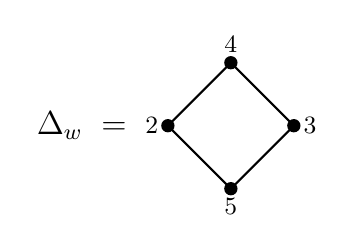
\begin{tikzpicture}[scale=0.4, vtx/.style={circle,fill=black,inner sep=1.7pt}]
      \coordinate (v2) at (-2,0);
      \coordinate (v4) at (0,2);
      \coordinate (v3) at (2,0);
      \coordinate (v5) at (0,-2);
      \draw[thick] (v2) -- (v4) -- (v3) -- (v5) -- cycle;
      \node[vtx] at (v2) {}; \node[vtx] at (v4) {};
      \node[vtx] at (v3) {}; \node[vtx] at (v5) {};
      \node[left]  at (v2) {\small $2$};
      \node[above] at (v4) {\small $4$};
      \node[right] at (v3) {\small $3$};
      \node[below] at (v5) {\small $5$};
      \node[anchor=east] at (-3,0) {\large $\Delta_w \;=$};
    \end{tikzpicture}
    \end{center}
    the join of the two-point complex on $\{2,3\}$ with the two-point complex on
    $\{4,5\}$.
\end{example}
As one would hope, the Bruhat order carries over into containment of simplicial complexes.

\begin{proposition}
\label{prop:Inclusion}
    Given $v,w\in S_n(\calP)$, the following are equivalent:
    \begin{itemize}
        \item $v\leq w$,
        \item $i(w) \leq i(v)$, $j(v)\leq j(w)$, if $i(v)=i(w)$ then $p(v)\leq p(w)$, and if $j(v)=j(w)$ then $q(w) \leq q(v)$,
        \item $\Delta_v\subseteq \Delta_w$.
    \end{itemize}
\end{proposition}
\begin{proof}
    We first show the top two bullets points are equivalent. Suppose $v,w\in S_n(\calP)$ such that $v\leq w$. Then $r_v(p,q) \geq r_w(p,q)$ for all $p,q$. Since for all $\ell<i(w)$, $r_v(\ell,\ell)\geq r_w(\ell,\ell) = \ell$, then $v$ must have fixed points up to index $i(w)-1$, meaning $i(v)\geq i(w)$. A similar argument shows $j(w)+1,\dots,n$ must be fixed points of $v$ so $j(v)\leq j(w)$.
    Suppose $i(v)=i(w)$, and set $i$ to be this common value. Then $i=r_v(p(v),i) \geq r_w(p(v),i)$ implies that the position of $i$ in $w$ is at or to the right of $p(v)$, meaning $p(w) \geq p(v)$. Supposing $j\coloneqq j(v)=j(w)$, since $r_v(q(w)-1,j-1)\geq r_w(q(w)-1,j-1) = q(w)-1$, this forces $v(\ell)\leq j-1$ for all $\ell<q(w)-1$, which implies $j$ must be weakly to the right of position $q(w)-1$, so $q(v)\geq q(w)$.
    Conversely, suppose $v,w\in S_n(\calP)$ and the three conditions hold. Then we have $r_v(a,b)= r_w(a,b)$ automatically for all $(a,b)$ except for those in $[i(w),j(w)-1]\times [i(w),j(w)-1]$. Thus, we may assume without loss of generality that $i(w)=1$ and $j(w)=n$, and we only need to check the inequality for $(a,b)$ in the square $[i(v),j(v)-1]\times [i(v),j(v)-1]$.
    It can be checked that for any $a,b<n$, 
    \[
    r_w(a,b) = \delta_{p(w)\leq a} + \max(0,a+b-n+1-\delta_{p(w)\leq a} - \delta_{q(w)\leq a})
    \]
    and shifting this formula by $i(v)-1$, we get
    \begin{align*}
    r_v(a,b) 
    & = i(v)-1 + \delta_{p(v)\leq a} + \max(0,(a-i(v)+1) \\ 
    & + (b-i(v)+1) - (j(v)-i(v)+1)+1 - \delta_{p(v)\leq a} - \delta_{q(v)\leq a}).\\
    &= i(v)-1 + \delta_{p(v)\leq a} + \max(0,a+b-j(v)-i(v)+2 - \delta_{p(v)\leq a} - \delta_{q(v)\leq a}).
    \end{align*}
    When both nonzero maxima are achieved, we have $r_w(a,b) = a+b-n+1-\delta_{q(w)\leq a}$ and $r_v(a,b) = a+b-j(v)+1-\delta_{q(v)\leq a}$. Then $r_w(a,b)\leq r_v(a,b)$ follows easily from the fact that if $j(w)=n=j(v)$ then $q(w)\leq q(v)$. If the max in $r_w(a,b)$ is $0$, then we have $r_w(a,b) = \delta_{p(w)\leq a}$, which is less than or equal to $i(v)-1+\delta_{p(v)\leq a}$ since $i(w)=1=i(v)$ implies $p(v)\leq p(w)$. Finally, if the max in $r_v(a,b)$ is $0$, then $a+b+2-j(v)-\delta_{q(v)\leq a}<i(v) + \delta_{p(v)\leq a}$. Using this inequality, we see $r_v(a,b) = i(v)-1+\delta_{p(v)\leq a} \geq a+b-n+1-\delta_{q(w)\leq a} \geq r_w(a,b)$. Thus, $r_w(a,b)\leq r_v(a,b)$ for all $a,b$, and thus $v\leq w$.
    
    The fact that the second and third bullet points are equivalent follows easily from the definition of $\Delta_v$ in terms of its nonfaces.
\end{proof}

\subsection{Intersections of doubly pruned complexes}
Doubly pruned complexes are closed under intersection. We prove this, and then
describe explicitly the intersections that arise from an antichain in $S_n(\calP)$.
\begin{proposition}
\label{prop:intersection is doubly pruned}
    The intersection of two doubly pruned simplicial complexes on $[n]$ is doubly pruned.
\end{proposition}
\begin{proof}
    Let $\Delta_1$ and $\Delta_2$ be doubly pruned, and for $r\in\{1,2\}$ write the nonfaces of $\Delta_r$ as generated by the singletons $\{k\}$ with $k\in[n]\setminus[i_r,j_r]$ together with at most one interval $[i_r,p_r]$ and at most one interval $[q_r,j_r]$. 
    A subset of $[n]$ is a nonface of $\Delta_1\cap\Delta_2$ if and only if it is a nonface of $\Delta_1$ or a nonface of $\Delta_2.$ Thus, the nonfaces of the intersection are generated by the union of the two generating sets. 
    Set $I = \max\{i_1,i_2\}$ and $J = \min\{j_1,j_2\}$, so that $[i_1,j_1]\cap[i_2,j_2] = [I,J]$.

    If $I>J$, then every $k\in[n]$ lies outside $[i_1,j_1]$ or outside $[i_2,j_2]$, so every singleton is a nonface and $\Delta_1\cap\Delta_2 = \emptyset$, which is doubly pruned by \Cref{def: doubly pruned simplicial complexes}. Assume then that $I\leq J$. We know that the singleton generators of the intersection are the $\{k\}$ with $k\not\in[i_1,j_1]$ together with the $\{k\}$ with $k\notin[i_2,j_2],$ which means they are precicely the $\{k\}$ with $k\notin[I,J]$.

    Now consider the at most four interval generators.
    If $i_r<I$, then $i_r\not\in[I,J]$, so $\{i_r\}$ is a singleton generator of the intersection contained in $[i_r,p_r]$. Thus, $[i_r,p_r]$ is not a minimal nonface and may be discarded. It is analogous for $[q_r,j_r]$ when $j_r>J$. Each surviving interval generator, therefore, has left endpoint $I$ or right endpoint $J$.

    There are at most two surviving generators with left endpoint $I,$ and any two intervals sharing a left endpoint are nested, so at most one of them is minimal.
    The same argument applies to the at most two surviving generators with right endpoint $J$. Hence the minimal nonfaces of $\Delta_1\cap\Delta_2$ are the singletons $\{k\}$ with $k\notin[I,J]$, together with at most one interval $[I,p]$ and at most one interval $[q,J]$, so $\Delta_1\cap\Delta_2$ is doubly
    pruned.
\end{proof}

\begin{corollary}\label{cor: lattice}
    The collection of doubly pruned simplicial complexes on $[n]$ forms a lattice under containment of simplicial complexes, in which the meet of $\Delta_1$ and $\Delta_2$ is $\Delta_1\cap\Delta_2$ and the join is the smallest doubly pruned complex containing $\Delta_1\cup\Delta_2.$
\end{corollary}

\begin{proof}
    By \Cref{prop:intersection is doubly pruned}, the intersection of two doubly pruned simplicial complexes on $[n]$ is a doubly pruned simplicial complex, hence the poset of doubly pruned simplicial complexes is a meet-semilattice, in which the meet is given by intersection. Since there is a unique top element of the finite poset, namely the simplex supported on $[1,n]$, it is therefore a lattice \cite[Prop.~3.3.1]{StanleyEC1}. 
    The doubly pruned complexes containing both $\Delta_1$ and $\Delta_2$ form a nonempty finite collection, as it contains the simplexes supported on $[1,n],$ so their intersection is the smallest doubly pruned complex containing $\Delta_1\cup\Delta_2.$
\end{proof}

\begin{remark}
    The subposet $\{\Delta_w : w\in S_n(\calP)\}$ is not a lattice. Indeed, observe that meets and joins do not exist when $n=4$; see Figure~\ref{fig: s4 simplicial complex poset}.
\end{remark}

\begin{corollary}
\label{lem:double pruned intersections}
    Let $\{v,w\}\subseteq S_n(\calP)$ be an antichain such that $i(v)\geq i(w)$, and if they are equal $p(v)< p(w)$. Then the nonfaces of $\Delta_v\cap\Delta_w$  are generated by 
    \[1,\dots,i(v)-1,\qquad j(w)+1,\dots,n,\qquad [i(v),p(v)],  [q(w),j(w)].\]
\end{corollary}
\begin{proof}
    As the intersection, the nonfaces of $\Delta_v\cap \Delta_w$ are generated by the minimal nonfaces of $\Delta_v$ union the nonfaces of $\Delta_w$.
    Thus, the intersection's minimal nonfaces are generated by 
    \begin{itemize}
        \item $1,\dots,\max(i(v)-1,i(w)-1),$
        \item $\min(j(v)+1,j(w)+1),\dots,n,$ and
        \item $[i(v),p(v)], [q(v),j(v)],[i(w),p(w)], [q(w),j(w)].$
    \end{itemize}
    By assumption, $\max(i(v)-1,i(w)-1) = i(v)-1$.
    
    If $j(w)>j(v)$, then either ($i(v)>i(w)$ and  $j(w)>j(v)$) or ($i(v)=i(w)$, $p(v)< p(w)$, and  $j(w)>j(v)$).
    In either case, by \Cref{prop:Inclusion}, $\Delta_v\subseteq  \Delta_w$, so $v\leq w$ which violates the assumption that they are an antichain.
    Thus, $\min(j(v)+1,j(w)+1)=j(w)+1$.
    If $i(w)<i(v)$, then $\{i(w)\}$ is a minimal nonface of $\Delta_v$ strictly contained in $[i(w),p(w)]$.
    If $i(w)=i(v)$, then $p(v)<p(w)$ so $[i(v),p(v)]$ is a minimal nonface of $\Delta_v$ strictly contained in $[i(w),p(w)]$.
    In either case, $[i(w),p(w)]$ is not a minimal nonface of the intersection.
    If $j(w)<j(v)$, then $j(v)$ is a minimal nonface of $\Delta_w$ strictly contained in $[q(v),j(v)]$.
    If $j(w)=j(v)$ and $q(w)\leq q(v)$, then $v\leq w$ by \Cref{prop:Inclusion} which violates the assumption that the pair is an antichain.
    If $j(w)=j(v)$ and $q(w)> q(v)$,
    then $[q(w),j(w)]$ is a minimal nonface of $\Delta_w$ strictly contained in $[q(v),j(v)]$.
    In both possible cases, $[q(v),j(v)]$ is not a minimal nonface of the intersection.
    Thus, the (minimal) nonfaces of $\Delta_v\cap \Delta_w$ are generated by
    \[1,\dots,i(v)-1,\qquad j(w)+1,\dots,n,\qquad [i(v),p(v)],  [q(w),j(w)].\qedhere\]
\end{proof}


\begin{corollary}
    \label{lem:antichain ordering}
    Let $\calW = \{w_1,\dots,w_m\} \subseteq S_n(\calP)$ be an antichain ordered lexicographically by the tuples \([i(w_k),j(w_k),-p(w_k),-q(w_k)]\).
    Then for all $k\in [1,m-1]$
    \[\Delta_{w_k}\cap \Delta_{w_m}\subseteq \Delta_{w_{k+1}}\cap \Delta_{w_m}\quad\text{ and }\quad \Delta_{w_k}\cap \Delta_{w_1}\supseteq \Delta_{w_{k+1}}\cap \Delta_{w_1}.\]
\end{corollary}
\begin{proof}
    As the inclusion $\Delta_{w_{m-1}}\cap \Delta_{w_m} \subseteq \Delta_{w_m}\cap \Delta_{w_m}$ is immediate, let $k\in[1,m-2]$.
    In order to conclude the inclusion $\Delta_{w_k}\cap \Delta_{w_m}\subseteq \Delta_{w_{k+1}}\cap \Delta_{w_m}$, it suffices to show that a set which generates the nonfaces of $\Delta_{w_k}\cap \Delta_{w_m}$ generates a set that generates the nonfaces of $\Delta_{w_{k+1}}\cap \Delta_{w_m}$.
    
    By the ordering either $i(w_m)> i(w_k)$ or, if they are equal, then $j(w_m)\geq j(w_k)$.
    If $i(w_m)= i(w_k)$ and $j(w_m)= j(w_k)$, then $-p(w_m)\geq -p(w_k)$; if those were equal, $\calW$ would not be an antichain so $p(w_k)> p(w_m)$.
    If $i(w_m)= i(w_k)$ and $j(w_m)> j(w_k)$, then in order for $\calW$ to be an antichain, $p(w_k)> p(w_m)$.
    Thus, in all cases, we may apply \Cref{lem:double pruned intersections}, and so the nonfaces of $\Delta_{w_k}\cap \Delta_{w_m}$
    \[1,\dots,i(w_m)-1,\qquad j(w_k)+1,\dots,n,\qquad [i(w_m),p(w_m)],  [q(w_k),j(w_k)].\]
    The exact same argument works replacing $k$ with $k+1$, and so the  nonfaces of $\Delta_{w_{k+1}}\cap \Delta_{w_m}$
    \[1,\dots,i(w_m)-1,\qquad j(w_{k+1})+1,\dots,n,\qquad [i(w_m),p(w_m)],  [q(w_{k+1}),j(w_{k+1})].\]
    In order to conclude the inclusion from those lists, it suffices to show that the first list generates the second list.
    In other words, it suffices to show that $j(w_k)\leq j(w_{k+1})$ and if they are equal, then $q(w_k)\geq q(w_{k+1})$ for $k\leq m-2$.
    By the ordering $i(w_k)\leq i(w_{k+1})$.
    If $i(w_k)= i(w_{k+1})$, then by the ordering $j(w_k)\leq j(w_{k+1})$.
    If $i(w_k)< i(w_{k+1})$ and $j(w_k)>j(w_{k+1})$, then $w_{k+1}\leq w_k$ by \Cref{prop:Inclusion}, so if $i(w_k)< i(w_{k+1})$, then $j(w_k)\leq j(w_{k+1})$.
    In either case, we have $j(w_k)\leq j(w_{k+1})$.
    If $j(w_k)< j(w_{k+1})$, then the conclusion holds, so we assume $j(w_k)= j(w_{k+1})$.
    It now suffices to show $q(w_k)\geq q(w_{k+1})$.
    As $i(w_k)\leq i(w_{k+1})$ by the ordering, we deal with it in two cases depending on if that is an equality or not.
    
    We deal with the equality case first.
    If $i(w_k)= i(w_{k+1})$, then as $j(w_k)= j(w_{k+1})$, by the ordering $p(w_k)\geq p(w_{k+1})$.
    If $p(w_k)= p(w_{k+1})$, then they are comparable by \Cref{prop:Inclusion} as the $i$ and $j$ coordinates were already equal, which is impossible so $p(w_k)> p(w_{k+1})$.
    If $p(w_k)> p(w_{k+1})$ and $q(w_k)\leq q(w_{k+1})$, then they are again comparable by \Cref{prop:Inclusion}, so $q(w_k)>  q(w_{k+1})$.
    Now we deal with the case of a strict inequality, i.e., $i(w_k)< i(w_{k+1})$.
    Recall we still have $j(w_k)= j(w_{k+1})$.
    If $q(w_k)\leq q(w_{k+1})$, then they are again comparable by \Cref{prop:Inclusion}, so $q(w_k)>  q(w_{k+1})$.
    
    An entirely symmetric argument proves the other inclusion.
\end{proof}